\documentclass[11pt]{scrartcl}
\usepackage[utf8]{inputenc}
\usepackage{amsmath, amssymb, amsthm, bbm}
\usepackage{booktabs, verbatim, graphicx, framed, gensymb}
\usepackage[sexy, hints]{evan}
\newcommand{\ca}[1]{\mathrm{#1}}
\title{Physics, Master Document}
\author{Anay Aggarwal}

\begin{document}

\maketitle
\section{Jamboards}
\href{https://jamboard.google.com/d/1uoYdMKXinEdf1\_fIV\_Um4zPiH8XeXSZzDs1etD-xgbI/viewer?f=0}{Statics} \newline
\href{https://jamboard.google.com/d/1ajkcgySLsFFmAIlD7kHRhOTfPmT233VM9uvkb6ygHFg/viewer?f=0}{Forces} \newline
\href{https://jamboard.google.com/d/19tQ1\_l9Pz5J62Dyj3KkGLjumSymWhyoXW8kS4kQQBSg/viewer?f=0}{More Forces} \newline
\href{https://jamboard.google.com/d/1MbDdIBIItbUHffvw165ii3ZKFlsYYW7sVqZbw3JTE5k/viewer?f=0}{Finishing Chapter 3} \newline
\href{https://jamboard.google.com/d/1dbo9FVwQZNCMXaT9OfHmJFNlvY1AcgZkJbSVOeSiLaU/viewer?f=0}{Oscillations} \newline
\href{https://jamboard.google.com/d/1a9brHy7W-hm7C\_LCcwz4QAHZM4OQ06tv0LuvaHiV9q0/viewer?f=0}{Finishin Ch. 4}
\newpage
\section{Statics}
The term "statics" means stationary. In a static system, no objects have any acceleration.
This means that two things are true:
\begin{itemize}
  \item The net force on the system is $0$.
  \item The net torque (spin) on the system is $0$.
\end{itemize}
So when solving a statics problem, draw the free-body diagram and balance forces \& torque.
There are $4$ main forces to understand:
\begin{itemize}
  \item Tension. Tension is force pulling on a point in a rope. For a massless rope, this force is the same to the left and to the right
    at any instantaneous spot in the rope, even if it is bent around a pulley, etc. Ropes with mass are trickier to deal with, the general
    idea is that tension is a function of a point on the rope.
  \item Normal force is a force opposing a surface, perpendicular to that surface. Think of it as like a spring.
  \item Friction is force opposing motion. The brief run-down is that kinetic friction satisfies $f_k=\mu_k N$ and static friction satisfies
    $f_s\le \mu_s N$.
  \item Gravity. The gravitational force between two bodies with masses $M,m$ and distance $R$ is
    $$F=\frac{GMm}{R^2}$$
    Where $G$ is a constant. For the earth, $\frac{GM}{R^2}=g$, hence the force is $mg$ downward in our reference frame.
\end{itemize}
On to problems.
\begin{example}
  [2.1 Red Book]
  A rope with length $L$ and mass density per unit length $\rho$ is suspended
  vertically from one end. Find the tension as a function of height along the rope.
\end{example}
\begin{soln}
  Consider an instant in the rope. The force is $T(y)$ downward and
  $T(y+\ca{dy})$ upward. The force of gravity is $\rho g\ca{dy}$. The system is static,
  so newton's second law tells us that the net force is zero. Therefore,
  $$T(y+\ca{dy})-T(y)-\rho g\ca{dy}=0 \implies T(y+\ca{dy})=T(y)+\rho g\ca{dy}$$
  $$\frac{T(y+\ca{dy})-T(y)}{\ca{dy}}=\rho g$$
  $$T'(y)=\rho g$$
  $$T(y)=\int \rho g \ca{dy}=\rho g y$$
\end{soln}
\begin{example}
  [2.2 Red Book]
  A block sits on a plane that is inclined at an angle $\theta$.
  Assume that the friction force is large enough to keep the block at rest.
  What are the horizontal components of the friction and normal forces
  acting on the block? For what $\theta$ are these horizontal components
  maximum?
\end{example}
\begin{soln}
  Drawing axes parallel to the hypotenuse of the ramp, we get that
  $$N=mg\cos(\theta)$$
  $$f_s=mg\sin(\theta)$$
  The problem asks for the horizontal component with normal axes, which is
  just $N\sin\theta=f_s\cos\theta=mg\sin\theta\cos\theta=\frac{mg\sin(2\theta)}{2}$.
  This attains its maximum $\frac{mg}{2}$ at $\theta=45^{\degree}$.
\end{soln}
\newpage
\begin{example}
  [2.3 Red Book]
  A frictionless tube lies in the vertical plane and is in the shape
  of a function that has its endpoints at the same height but is otherwise
  arbitrary. A chain with uniform mass per unit length lies in the tube from
  end to end. Show that the chain doesn't move.
\end{example}
\begin{soln}
  Consider an infinitesimal piece of the chain. We want the net force along
  the direction of the tube to be $0$, so the sum of the forces
  for each piece should be $0$. Since the pieces are infinitesimal,
  we can sum them with an integral. In order words, we want to show that
  $$\int a \ca{dm}=0$$
  At infinitesimals, stuff is easy to work with, because we can assume the
  piece of the chain to be a line. Let the function of the tube be $f(x)$.
  Consider the following diagram.
  \begin{center}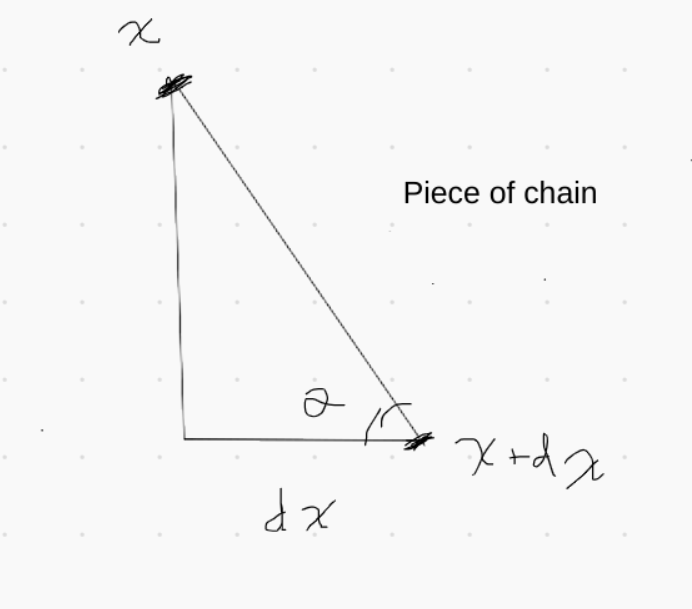
\includegraphics[scale=0.3]{Diagram1.png}\end{center}
    Notice that $f'(x)$ is defined to be the change in the y direction at
    an instantaneous moment, i.e. the other leg of the triangle is $f'(x)dx$.
    The hypotenuse, or length of the chain is then $\sqrt{f'(x)^2+1}dx$.
    Hence the mass is $\rho\sqrt{f'(x)^2+1}dx$.
    Since it is a ramp, notice that the force downward is $mg\sin\theta$.
    Thus by newton's laws
    $$ma=-mg\sin\theta\implies a=-g\sin\theta$$
    But $\sin\theta=\frac{f'(x)dx}{\sqrt{f'(x)^2+1}dx}=\frac{f'(x)}{\sqrt{f'(x)^2+1}}$.
    Hence it suffices to show that
    $$\int \frac{f'(x)}{\sqrt{f'(x)^2+1}}\rho\sqrt{f'(x)^2+1}dx=0$$
    $$\int \rho f'(x)=0$$
    Which is true due to the fact that $f(x_{\ca{initial}})=f(x_{\ca{final}})$.
\end{soln}
\begin{example}
  [2.4 Red Book]
  A book of mass $M$ is positioned against a vertical wall. The coefficient
  of friction between the book and the wall is $\mu$. You wish to keep the
  book from falling by pushing on it with a force $F$ applied to an angle
  $\theta$ with respect to the horizontal.
  \begin{itemize}
    \item For a given $\theta$, what is $\min F$?
    \item For what $\theta$ is $\min F$ minimized? What is the said minimum?
    \item What is the limiting value of $\theta$ such that there doesn't
      exist an $F$?
  \end{itemize}
\end{example}
\begin{soln}
  The upward force applied is $F\sin\theta$. The downward force from the book
  is $Mg$. The last force to worry about is friction, which we will denote by
  $f_s$. We have $f_s\le \mu N=\mu F\cos\theta$. Hence we have
  $$F\sin\theta+\mu F\cos\theta\ge Mg$$
  $$F\ge \frac{Mg}{\sin\theta+\mu\cos\theta}$$
  Solving the first part. For the second, we wish to maximize
  $$\sin\theta+\mu\cos\theta$$
  Taking the derivative w.r.t $\theta$, this is
  $$\cos\theta-\mu\sin\theta=0\to \theta=\arctan\left(\frac{1}{\mu}\right)$$
  Therefore we get
  $$\sin\theta=\frac{1}{\sqrt{\mu^2+1}}$$
  $$\cos\theta=\frac{\mu}{\sqrt{\mu^2+1}}$$
  Hence $\sin\theta+\mu\cos\theta=\sqrt{\mu^2+1}$. Therefore,
  $$\min\min F=\frac{Mg}{\sqrt{\mu^2+1}}$$
  Onto the last part, there doesn't exist an $F$ if and only if
  $$\sin\theta+\mu\cos\theta\le 0$$
  The limiting value is $\sin\theta+\mu\cos\theta=0$. This implies that
  said $\theta=\arctan(-\mu)$.
\end{soln}
\begin{example}
  [2.5 Red Book]
  A rope with length $L$ and mass density per unit length $\rho$ lies on a plane
  inclined at an angle $\theta$. The top end is nailed to the plane, and the
  coefficient of friction between the rope and the plane is $\mu$. What are
  the possible values for the tension at the top of the rope?
\end{example}
\begin{soln}
  The mass of the rope is $\rho L$. Choose the $x$ and $y$ axes as normally,
  along the plane. Hence the force in the $x$ direction is $\rho Lg\sin\theta$.
  The normal force is $N=\rho Lg\cos\theta$, hence the force of static friction is
  $$f_s\le \mu N=\mu \rho Lg\cos\theta$$
  Thus
  $$T+\mu\rho Lg\cos\theta\ge \rho Lg\sin\theta$$
  $$T\ge (\rho Lg)(\sin\theta-\mu\cos\theta)$$
  But we also get the upper bound
  $$T\le (\rho Lg)(\sin\theta+\mu\cos\theta)$$
  The same way.
\end{soln}
\begin{example}
  [2.6 Red Book]
  Consider the two problems
  \begin{itemize}
    \item A disk of mass $M$ and radius $R$ is help up by a massless string.
      The surface of the disk is frictionless. What is the tension
      in the string? What is the normal force per unit length that the string
      applies on the disk?
    \item Let there now be friction between the disk and the string, with
      coefficient $\mu$. What is the smallest possible tension in the string
      at its lowest point?
  \end{itemize}
\end{example}
\begin{soln}
  The solutions are as follows.
  \begin{itemize}
    \item Notice that there is a tension $T$ upward in each end of the string,
      hence $2T=Mg\to T=\frac{Mg}{2}$. At small instants in the rope, the normal
      force is essentially just the tension. For an angle $\theta$, the normal
      force is $N\theta$ and the length is $R\theta$, hence we want
      $$\frac{N\theta}{R\theta}=\frac{N}{R}=\frac{Mg}{2R}$$
    \item Using the rope wrapped around pole example,
      $$T(\frac{\pi}{2})\le T(0)e^{\mu\frac{\pi}{2}}$$
      $$T(0)\ge \frac{Mg}{2}e^{-\mu\frac{\pi}{2}}$$
  \end{itemize}
\end{soln}
\begin{example}
  [2.7 Red Book]
  Each of the following planar objects is places (see figure $2.13$ in book)
  between two frictionless circles of radius $R$. The mass densite per unit area
  of each object is $\sigma$, and the radii to the points of contact make an
  angle $\theta$ with the horizontal. For each case, find the horizontal
  force that must be applied to the circles to keep them together. For
  what $\theta$ is this force maximum or minimum?
\end{example}
\begin{soln}
  For the first one, a bit of angle chasing (note the kites) yields that the angle at the apex of the triangle is $2\theta$.
  Hence by the sine area formula, it's area is $L^2\sin(2\theta)\frac{1}{2}=L^2\sin\theta\cos\theta$. Hence the mass is $\sigma L^2\sin\theta\cos\theta$.
  Let $F_{CT}$ be the force from the circle on the triangle. Notice that
  $$2F_{CT}\sin\theta=mg=\sigma g L^2\sin\theta\cos\theta$$
  $$F_{CT}=\frac{\sigma g L^2\cos\theta}{2}$$
  We desire
  $$F_{CT}\cos\theta=\frac{L^2\cos^2\theta \sigma g}{2}$$
  Similarly for the other cases, the answer is just $\frac{mg\cos\theta}{2\sin\theta}$.
  And $m=\sigma A$, where $A$ is the area. To find the area of the rectangle, simply draw in the isosceles trapezoid.
  The unkown side is just $2R(1-\cos\theta)$, hence the area is $2RL(1-\cos\theta)$ and the mass is $2RL\sigma(1-\cos\theta)$. Therefore, the answer is
  $$RL\sigma (1-\cos\theta)\cot\theta$$
  The last case is a circle. It's a fun geometry puzzle to figure out the area of this. Connect the centers.
  Let the small circle have radius $r$. Then
  $\frac{r+R}{\sin\theta}=\frac{2R}{\sin(180-2\theta)}=\frac{2R}{\sin(2\theta)}=\frac{R}{\sin\theta\cos\theta}$
  $$r=R\left(\frac{1}{\cos\theta}-1\right)$$
  And hence the answer is $\pi g R^2\left(\frac{1}{\cos\theta}-1\right)^2\sigma\frac{\cos\theta}{2\sin\theta}$.
  This is equivalent to
  $$\frac{\sigma g\pi R^2(1-\cos\theta)^2}{\sin(2\theta)}$$
  Now, we must maximize each one. Fortunately this isn't too difficult because
  we only must maximize the part that is dependent on $\theta$.
  \begin{itemize}
    \item The first case is to maximize $\cos\theta$, which occurs at
      $\theta=0$. The minimum is at $\theta=\frac{\pi}{2}$.
    \item The second case is to maximize $(1-\cos\theta)\cot\theta$. This is
      $$f(\theta)=\frac{\cos\theta-\cos^2\theta}{\sin\theta}$$
      Using the quotient rule,
      $$f'(\theta)=\cos^3(\theta)-2\cos(\theta)+1=0$$
      Hence
      $$\theta=\arccos\left(\frac{-1+\sqrt{5}}{2}\right)$$
      The minimimum is at both $\theta=\frac{\pi}{2}, 0$.
    \item The third case goes to infinity as $\theta$ approaches
      45 degrees. It's minimized at $\theta=0$.
  \end{itemize}
\end{soln}
\begin{example}
  [2.8 Red Book]
  Consider the two problems:
  \begin{itemize}
    \item A chain with uniform mass density per unit length hangs
      between two given points on two walls. Find the general shape of the
      chain. Aside from an arbitrary additive constant, the function
      describing the shape should contain one unknown constant.
    \item The unknown constant in your answer depends on the horizontal
      distance $d$ between the walls, and the vertical distance $\lambda$
      between the support points, and the length $\ell$ of the chain. Write
      the constant in terms of these quantities.
  \end{itemize}
\end{example}
\begin{soln}
\end{soln}
\begin{example}
  [2.9 Red Book]
  A chain with uniform mass density per unit length hands between two supports located
  at the same height, a distance $2d$ apart. What should the length of the chain be so that
  the magnitude of the force at the supports is minimized?
\end{example}
\begin{soln}
\end{soln}
\newpage
\section{Forces}
\begin{example}
  [3.1]
  A massless pulley hangs from a fixed support. A massless string connnecting
  two masses, $m_1$ and $m_2$, hangs over the pulley (see Fig. 3.11).
  Find the acceleration of the masses and the tension in the string.
\end{example}
\begin{soln}
  Note that the acceleration is constant, so
  $$T-m_1g=m_1a$$
  $$T-m_2g=-m_2a$$
  Which, when solved, gives
  $$a=\frac{m_2g-m_1g}{m_2+m_1}, T=\frac{2m_1m_2g}{m_2+m_1}$$
\end{soln}
\begin{example}
  [3.2]
  A double Atwood's machine is shown in Fig. 3.12, with masses $m_1, m_2, m_3$.
  Find the acceleration of each mass.
\end{example}
\begin{soln}
  The equations are
  $$2T-m_1g=m_1a_1, T-m_2g=m_2a_2, T-m_3g=m_3a_3$$
  And then from conservation of string,
  $$a_1=\frac{-a_2-a_3}{2}$$
  And the accelerations can be solved for as
  $$a_1=g\frac{4m_2m_3-m_1m_2-m_1m_3}{4m_2m_3+m_1m_2+m_1m_3}$$
  $$a_2=-g\frac{4m_2m_3+m_1m_2-3m_1m_3}{4m_2m_3+m_1m_2+m_1m+3}$$
  $$a_3=-g\frac{4m_2m_3+m_1m_3-3m_2m_1}{4m_2m_3+m_1m_2+m_1m_3}$$
\end{soln}
\begin{example}
  [3.3]
  Consider the infinite Atwood’s machine shown in Fig. 3.13. A string
  passes over each pulley, with one end attached to a mass and the other
  end attached to another pulley. All the masses are equal to m, and all
  the pulleys and strings are massless. The masses are held fixed and then
  simultaneously released. What is the acceleration of the top mass? (You
  may define this infinite system as follows. Consider it to be made of
  N pulleys, with a nonzero mass replacing what would have been the
  (N + 1)th pulley. Then take the limit as $N\to\infty$.)
\end{example}
\begin{soln}
  For a finite system, we get the equations
  $$2T-mg=ma_1$$
  $$2T-mg=ma_2$$
  $$\cdots$$
  $$T-mg=ma_{n}$$
  $$T-mg=ma_{n+1}$$
  Conservation of string equations aren't needed yet. We get that
  $$g+a_1=g+a_2=\cdots=g+a_{n-1}=2g+2a_n=2g+2a_{n+1}$$
  So $a_1=a_2=a_3...=a_{n-1}$. But by conservation of string, we get that
  $$a_1=a_{n-1}=-\frac{a_n+a_{n+1}}{2}=-a_n$$
  $$a_1=2a_n+g$$
  $$a_n=-\frac{g}{3}$$
  $$a_1=\frac{g}{3}$$
\end{soln}
\begin{example}
  [3.4]
  $N+2$ equal masses hand from a system of pulleys, as shown in Fig. 3.14.
  What are the accelerations of all the masses?
\end{example}
\begin{soln}
  We have that
  $$T-mg=ma$$
  $$2T-mg=ma_1$$
  But $2a_1N=-2a$ by conservation of string. Hence
  $$a=-\frac{Ng}{2N+1}, a_1=\frac{g}{2N+1}$$
\end{soln}
\begin{example}
  [3.5]
  Consider the system of pulleys shown in FIg. 3.15. The string (which is a loop with no ends)
  hangs over $N$ fixed pulleys that circle around the underside of a ring.
  $N$ masses, $m_1, m_2,\cdots, m_N$ are attached to $N$ pulleys that hang
  on the string. What are the accelerations of all the masses.
\end{example}
\begin{soln}
  We get
  $$2T-m_k g=m_ka_k$$
  For each $k$. Since the masses are placed around a ring,
  $$a_1+a_2+...+a_N=0$$
  But $a_k=\frac{2T-m_k g}{m_k}$. Hence
  $$\sum a_k=\sum \frac{2T}{m_k}-g=2T\sum \frac{1}{m_k}-Ng=0$$
  $$T=\frac{Ng}{2\sum \frac{1}{m_k}}$$
  And hence
  $$a_k=\frac{\frac{Ng}{\sum \frac{1}{m_k}}-m_k g}{m_k}$$
\end{soln}
\begin{example}
  [3.6]
  Problems are as follows:
  \begin{itemize}
    \item A block starts at rest and slides down a frictionless plane
      inclined at an angle $\theta$. What should $\theta$ be so that the block
      travels a given horizontal distance in the minimum amount of time.
    \item Same question, now there is a coefficient of friction $\mu$.
  \end{itemize}
\end{example}
\begin{soln}
  Consider the following solutions.
  \begin{itemize}
    \item Suppose the distance is $d$ and the time is $t$. The force downward
      has magnitude $mg$, so the force down the plane has magnitude
      $mg\sin\theta$. Hence the acceleration is $g\sin\theta$. The
      initial velocity is zero, so we can use
      $$d=\frac{1}{2}at^2$$
      $$g\sin\theta=\frac{2d}{t^2}$$
      $$\theta=\arcsin\left(\frac{2d}{t^2 g}\right)$$
      We want theta such that $t$ is minimized, so $\theta=45$.
    \item Same thing, except the acceleration is now $g\sin\theta-\mu g\cos\theta$.
      Hence
      $$g\sin\theta-\mu g\cos\theta=\frac{2d}{t^2}$$
      $$\sin\theta-\mu\cos\theta=\frac{2d}{t^2 g}$$
      For now, define $y:=\frac{2d}{t^2 g}$.
      Let $x=\sin\theta$. We want to solve
      $$x-y=\mu \sqrt{1-x^2}$$
      $$(x-y)^2=\mu^2(1-x^2)$$
      $$x^2-2xy+y^2=\mu^2-x^2\mu^2$$
      $$x^2(1+\mu^2)-2xy+y^2-\mu^2=0$$
      $$x=\frac{2y\pm 2\sqrt{y^2+(1+\mu^2)\mu^2}}{2+2\mu^2}$$
      $$x=\frac{y\pm \sqrt{y^2+\mu^2+\mu^4}}{1+\mu^2}$$
      Taking only the positive value,
      $$\theta=\arcsin\left(\frac{\frac{2d}{t^2g}+\sqrt{\frac{4d^2}{t^4g^2}+\mu^2+\mu^4}}{1+\mu^2}\right)$$
      To minimize $t$, we want the value in the parentheses to be fixed as a small value,
      specifically $\theta=\frac{\arctan(-\frac{1}{\mu})}{2}$ (which can be obtained with nasty calculations after taking the derivative).
  \end{itemize}
\end{soln}
\begin{example}
  [3.8]
  A block of mass $m$ is held motionless on a frictionless plane of mass $M$
  and angle of inclination $\theta$ (see Fig. 3.16). The plane rests on a
  frictionless horizontal surface. The block is released. What is the
  horizontal acceleration of the plane?
\end{example}
\begin{soln}
  Note that we have
  $$mg-N\cos\theta=ma_y$$
  $$N\sin\theta=ma_x=Ma'_x$$
  Hence $N=\frac{mg-ma_y}{\cos\theta}=\frac{ma_x}{\sin\theta}$.
  Thus $a_x=(g-a_y)\tan\theta$.
  In addition, the ratio of the y accleration to the x acceleration must
  remain $\tan\theta$, so
  $$a_y=(a_x+a'_x)\tan\theta$$
  $$mg-N\cos\theta=N\sin\theta+\frac{m}{M'}N\sin\theta$$
  $$mg-N\cos\theta=N\sin\theta(\frac{M'+m}{M'})$$
  A bunch of algebra gives
  $$a'_x=\frac{mg\sin\theta\cos\theta}{M+m\sin^2\theta}$$
\end{soln}
\begin{example}
  [3.9]
  A particle of mass $m$ is subject to a force $F(t)=ma_0e^{-bt}$.
  The initial position and speed are zero. Find $x(t)$.
\end{example}
\begin{soln}
  The magnitude of the acceleration is hence $a=a_0e^{-bt}$.
  Notice
  $$\frac{\mathrm{d}^2x}{\mathrm{d}t^2}=a_0e^{-bt}$$
  $$x=\int \int a_0e^{-bt}\ca{dt}\ca{dt}$$
  Now,
  $$\int a_0e^{-bt}\ca{dt}=a_0\int e^{-bt}\ca{dt}=\frac{a_0e^{-bt}}{-b}+C_1$$
  The initial speed is zero so
  $$C_1=\frac{a_0}{b}$$
  Then
  $$x=\frac{a_0e^{-bt}}{b^2}+\frac{a_0}{b}t+C_2$$
  Now, the initial position is zero, so likewise we find
  $$C_2=-\frac{a_0}{b^2}$$
  Thus
  $$x(t)=\frac{a_0e^{-bt}}{b^2}+\frac{a_0}{b}t-\frac{a_0}{b^2}$$
\end{soln}
\begin{example}
  [3.10]
  Same question just initial position is $x_0$ and $F(x)=-kx$.
\end{example}
\begin{soln}
  We have that
  $$mv\frac{\ca{dv}}{\ca{dx}}=-kx$$
  $$mv\ca{dx}=-kx\ca{dx}$$
  $$\int_{x_0}^x -kx\ca{dx}=\int_0^v mv\ca{dv}$$
  $$kx_0^2-kx^2=mv^2$$
  Employing $\omega=\sqrt{\frac{k}{m}}$, this is
  $$v=\omega\sqrt{x_0^2-x^2}$$
  $$\int_{x_0}^x\frac{1}{\sqrt{x_0^2-x^2}}\ca{dx}=\int_0^t \omega\ca{dt}$$
  $$\int_{x_0}^x \frac{1}{\sqrt{x_0^2-x^2}}\ca{dx}=\omega t$$
  Substitute $x=x_0\cos\theta$, then
  $$\int_{0}^{\theta} \frac{1}{x_0\sin\theta}\ca{dx}=\int_{0}^{\theta} -\ca{d}\theta$$
  Hence $\theta=-\omega t$, and $x=x_0\cos(\omega t)$
\end{soln}
\begin{example}
  [3.11]
  A chain with length $\ell$ is held stretched out on a frictionless horizontal
  table, with a length $y_0$ hanging down through a hole in the table. The
  chain is released. As a function of time, find the length that hangs down
  through the hole (don’t bother with t after the chain loses contact with
  the table). Also, find the speed of the chain right when it loses contact
  with the table.
\end{example}
\begin{soln}
  Suppose the chain has density $\rho$. Suppose the chain
  has a length $y$ down the hole. Consider forces, we get the differential equation
  $$a=\frac{g}{\ell}y$$
  Which is the differential equation for SHM with $\omega=\sqrt{\frac{g}{\ell}}$ and
  without a factor of $i$. Hence the solution is
  $$y=y_0\cosh\left(\sqrt{\frac{g}{\ell}}t\right)$$
\end{soln}
\begin{example}
  [3.14]
  A ball is thrown at speed $v$ from zero height on level ground.
  At what angle should it be thrown so that the area
  under the trajectory is maximum?
\end{example}
\begin{soln}
  Notice that we have the parametrics
  $$y(t)=v_0\sin\theta t-\frac{1}{2}gt^2$$
  $$x(t)=v_0\cos\theta t$$
  We want to maximize
  $$\int_0^{2v_0\sin\theta g}y\ca{dx}=v_0\cos\theta\int_0^{2v_0\sin\theta g}y\ca{dt}$$
  $$=v_0\cos\theta\left(\frac{v_0\sin\theta t^2}{2}-\frac{gt^3}{6}\right)\Big|_{0}^{2v_0\sin\theta g}$$
  Which is
  $$\frac{v_0^2\sin\theta\cos\theta \frac{4v_0^2}{g^2}\sin^2\theta}{2}-v_0\cos\theta g\frac{8v_0^3\sin^3\theta g^3}{6}$$
  $$\frac{4v_0^4\sin^3\theta\cos\theta}{2g^2}-\frac{8v_0^4\sin^3\theta\cos\theta g^4}{6}$$
  Which is of the form $c\sin^3\theta\cos\theta$ for a fixed constant $c$ that doesn't
  depend on $\theta$. Thus it suffices to maximize $\sin^3\theta\cos\theta$.
  Let $x=\sin\theta$. This expression is then
  $$x^3\sqrt{1-x^2}=\sqrt{x^6-x^8}$$
  Hence it suffices to maximize $x^6-x^8$. The derivative of this is
  $$6x^5-8x^7=0\implies x=\frac{\sqrt{3}}{2}$$
  And $\sin\theta=\frac{\sqrt{3}}{2}$, so $\theta=60$ degrees.
\end{soln}
\begin{example}
  [3.15]
  A ball is thrown straight upward so that it reaches a height $h$.
  It falls down and bounces repeatedly. After each bounce, it returns to
  a certain fraction $f$ of its previous height. Find the total
  distance traveled, and also the total time, before it comes to rest.
  What is its average speed?
\end{example}
\begin{soln}
  The total distance is just
  $$2h(1+f+f^2+f^3+...)=\frac{2h}{1-f}$$
  For a distance $d$, the acceleration is $-g$, so the distance is $-\frac{1}{2}gt^2=-d$, so $t=\sqrt{\frac{2d}{g}}$.
  It takes the same amount of time to go back up so each one is $2\sqrt{\frac{2d}{g}}$. So we want
  $$2\sqrt{\frac{2h}{g}}+2\sqrt{\frac{2hf}{g}}+2\frac{\frac{2hf^2}{g}}+...=2\sqrt{\frac{2h}{g}}\left(1+\sqrt{f}+\sqrt{f^2}+...\right)$$
  $$=2\sqrt{\frac{2h}{g}}\frac{1}{1-\sqrt{f}}$$
  The average speed is then
  $$\frac{\frac{2h}{1-f}}{\frac{2\sqrt{\frac{2h}{g}}}{1-\sqrt{f}}}$$
  $$\frac{h(1-\sqrt{f})}{\sqrt{\frac{2h}{g}}(1-f)}$$
  $$\frac{h\sqrt{g}(1-\sqrt{f})}{\sqrt{2h}(1-f)}$$
\end{soln}
\begin{example}
  [3.17]
  A ball is thrown with speed $v$ from the edge of a cliff of height $h$.
  At what inclination angle should it be thrown so that it travels
  the maximum horizontal distance? What is this maximum distance?
  Assume that the ground below the cliff is horizontal.
\end{example}
\begin{soln}
  Suppose it's thrown at an angle $\theta$. The velocity horizontally is $v\cos\theta$.
  The velocity vertically is $v\sin\theta-gt$. Hence the change in horizontal distance is $v\sin\theta t-\frac{1}{2}gt^2$.
  The initial position is $h$, the final position is $0$, so the change must be $-h$. Hence
  $$\frac{1}{2}gt^2-v\sin\theta t+h=0$$
  $$t=\frac{v\sin\theta+\sqrt{v^2\sin^2\theta-2gh}}{g}$$
  Then the horizontal distance is
  $$\frac{v^2\sin\theta\cos\theta+\sqrt{v^4\sin^2\theta\cos^2\theta-2ghv^2\cos^2\theta}}{g}$$
  Which has maximum value $\frac{v^2}{g}\sqrt{1+\frac{2gh}{v^2}}$ at $\theta=\arcsin\left(\frac{1}{\sqrt{2+2gh/v^2}}\right)$.
\end{soln}
\begin{example}
  [3.25]
  The two problems:
  \begin{itemize}
    \item Find the acceleration of all the masses in Fig 3.18
    \item Same question, just remove the last mass
  \end{itemize}
\end{example}
\begin{soln}
  The two solutions:
  \begin{itemize}
    \item We have the equations
      $$T_k-m_k g=a_k$$
      $$T_k=\frac{T}{2^{k-1}}$$
      $$a_{n-1}=-\left(\frac{a_{n1}+a_{n2}}{2}\right)$$
      When solved, we get
      $$a_k=\frac{-3mg}{2^k}$$
    \item idk
  \end{itemize}
\end{soln}
\begin{example}
  [3.26]
  In the figure 3.19, find $M=f(m_1, m_2)$ such that it's stationary.
\end{example}
\begin{soln}
  From problem 2.2, we just want
  $$g\frac{4m_1m_2-M(m_1+m_2)}{4m_1m_2+M(m_1+m_2)}=0$$
  $$M=\frac{4m_1m_2}{m_1+m_2}$$
\end{soln}
\begin{example}
  [3.27]
  Find the acceleration of the two masses in Fig. 3.20.
\end{example}
\begin{soln}
  Drawing tensions, the first two equations are
  $$T-mg=ma_1$$
  $$4T-2mg=2ma_2\to 2T-mg=ma_2$$
  We have three unknowns, so we need an equation derived from conservation
  of string. Pushing the mass $m$ up a distance $d$, we see that
  the mass $2m$ goes down a distance $2d$ (by tracking). So
  $$x_1=2x_2$$
  $$a_1=-2a_2$$
  Which is our last equation. Solving, we get
  $$a_2=\frac{g}{5}, a_1=-\frac{2g}{5}$$
\end{soln}
\begin{example}
  [3.33]
  A block of mass m rests on a plane inclined at an angle $\theta$. The coefficient
  of static friction between the block and the plane is $\mu$. The plane is
  accelerated to the right with acceleration a (which may be negative);
  see Fig. 3.26. For what range of $a$ does the block remain at rest with
  respect to the plane? In terms of $\mu$, there are two special values of $\theta$;
  what are they, and why are they special?
\end{example}
\begin{soln}
  Balancing the forces in the horizontal direction,
  $$ma\cos\theta+mg\sin\theta=f_s\le \mu N=\mu mg\cos\theta$$
  $$a\le \mu g-g\tan\theta$$
  Also, $f_s\ge 0$, so $a\ge -g\tan\theta$. Hence
  $$a\in\left[-g\tan\theta, \mu g-g\tan\theta\right]$$
  I presume that the two "special values" of $\theta$ are the equality cases.
\end{soln}
\begin{example}
  [3.34]
  Three identical cylinders are arranged in a triangle as shown in Fig. 3.27,
  with the bottom two lying on the ground. The ground and the cylinders
  are frictionless. You apply a constant horizontal force (directed to the
  right) on the left cylinder. Let $a$ be the acceleration you give to the
  system. For what range of $a$ will all three cylinders remain in contact
  with each other?
\end{example}
\begin{soln}
  The equations are
  $$(N_1+N_2)\frac{\sqrt{3}}{2}=mg$$
  $$(N_1-N_2)\frac{1}{2}=ma$$
  $$a=\frac{F}{3m}$$
  where $N_1,N_2$ are the normal forces unto the top cylinder.
  The first two equations are from balancing forces, and the last one is trivial.
  In order to have minimum acceleration, no normal force must be there
  between the bottom two cylinders. Because then the bottom two cylinders have barely even touched yet. So, $N_2\frac{1}{2}=ma$. Solving gives
  $a=\frac{g}{3\sqrt{3}}$
  In order to have maximum acceleration, there must be no normal force between
  the right one and the top one (i.e. $N_2=0$). This is because after that
  contact is lost between those two cylinders. Solving, $a=\frac{g}{\sqrt{3}}$.
  Therefore,
  $$a\in \left[\frac{g}{3\sqrt{3}}, \frac{g}{\sqrt{3}}\right]$$
\end{soln}
\begin{example}
  [3.36]
\end{example}
\begin{soln}
\end{soln}
\begin{example}
  [3.37]
  A particle with mass $m$ is subject to $F(v)=-bv^2$. $x_0=0$. Find $x(t)$
\end{example}
\begin{soln}
  We have $a=\frac{\ca{dv}}{\ca{dt}}=-\frac{b}{m}v^2$.
  So
  $$\int \frac{1}{v^2}\ca{dx}=\int -\frac{b}{m}\ca{dt}=-\frac{b}{m}t$$
  Solving, $v=\frac{\ca{dx}}{\ca{dt}}=\frac{m}{bt}$. So,
  $$\int \ca{dx}=\int \frac{m}{bt}\ca{dt}$$
  $$x(t)=\frac{m}{b}\ln(t)$$
  Remembering $v_0$,
  $$x(t)=\frac{m}{b}\ln(t)+v_0t$$
\end{soln}
\begin{example}
  [3.43]
  Find the horizontal distance of projectile motion with $g(t)=\beta t$, and maximize this using $\theta$. Initial velocity is $v_0$.
\end{example}
\begin{soln}
  At an instant $t$, the horizontal speed is $$v_0\cos\theta$$ and the
  vertical speed is $$v_0\sin\theta-\beta t^2$$
  Hence the vertical distance is
  $$v_0\sin\theta t-\frac{t^3\beta}{3}$$
  upon integrating w.r.t $t$. Setting this equal to $0$,
  $$t=\sqrt{\frac{3v_0\sin\theta}{\beta}}$$
  So the total horizontal distance is
  $$\sqrt{\frac{3v_0^3\sin\theta\cos^2\theta}{\beta}}$$
  And hence it suffices to maximize $\sin\theta\cos^2\theta$.
  Let $x=\sin\theta$, then the expression is
  $$x(1-x^2)=x-x^3$$
  The derivative is $1-3x^2=0\implies x=\frac{1}{\sqrt{3}}$, so
  $\theta=\arcsin\left(\frac{1}{\sqrt{3}}\right)$
\end{soln}
\begin{example}
  [3.44]
  Newton gets angry at an apple, tries to chuck a rock at it but the apple falls out of the tree as he chucks the rock.
  It's his lucky day though, the rock hits the apple. Why?
\end{example}
\begin{soln}
  It's because the rock falls with acceleration $g$,
  and so does the apple, so they fall the same distance. If he aimed perfectly,
  the rock will hit the apple. It's easy to see mathematically.
\end{soln}
\begin{example}
  [3.47]
  You throw a ball with speed $v_0$ at a vertical wall, a distance $\ell$ away. At what angle should you throw the ball so that it hits the wall as high as
  possible? Assume $\ell<\frac{v_0^2}{g}$ (why?).
\end{example}
\begin{soln}
  The horizontal speed is $v_0\cos\theta$, so the time is $\frac{\ell}{v_0\cos\theta}$. So the vertical position is then
  $$\frac{v_0\sin\theta\ell}{v_0\cos\theta}-\frac{g\ell^2}{2v_0^2\cos^2\theta}$$
  $$\ell\tan\theta-\frac{g\ell^2}{2v_0^2} \frac{1}{\cos^2\theta}$$
  The derivative w.r.t $\theta$ is
  $$\ell\sec^2\theta-\frac{g\ell^2}{v_0^2}\tan\theta\sec^2\theta=0$$
  $$\tan\theta=\frac{v_0^2}{g\ell}$$
\end{soln}
\begin{example}
  [3.48]
  A cannon, when aimed vertically, is observed to fire a ball to a maximum
  height of L. Another ball is then fired with this same speed, but with the
  cannon aimed up along a plane of length L, inclined at an angle $\theta$, as
  shown in Fig. 3.31. What should $\theta$ be so that the ball travels the largest
  horizontal distance, d, by the time it returns to the height of the top of
  the plane?
\end{example}
\begin{soln}
  Suppose the initial speed is $v_0$. The time it takes to reach the
  max height is $t=\frac{v_0}{g}$. So the maximum height is
  $$\frac{v_0^2}{g}-\frac{v_0^2}{2g}=\frac{v_0^2}{2g}=L$$
  Suppose the velocity that the cannon is fired at is $v$. Then the time
  it takes is the difference of the two roots of
  $$vt-\frac{1}{2}gt^2=\frac{v_0^2\sin\theta}{2g}$$
  Which is just the discriminant, or
  $$\sqrt{v^2-v_0^2\sin\theta}$$
  So the total expression that we want to maximize is
  $$v\cos\theta\sqrt{v^2-v_0^2\sin\theta}$$
  So it suffices to maximize $v^4\cos^2\theta-v_0^2v^2\cos^2\theta\sin\theta$.
  Taking derivatives, we want
  $$-2\sin\theta\cos\theta=3\cos^3\theta-2\cos\theta$$
  $$-2\sin\theta=3\cos^2\theta-2$$
  Let $\sin\theta=x$. Then
  $$-2x=3(1-x^2)-2=3-3x^2-2=1-3x^2$$
  So $3x^2-2x-1=0$. Taking the positive root, $x=\frac{2+\sqrt{18}}{6}$.
  So the angle is
  $$\theta=\arcsin\left(\frac{2+\sqrt{18}}{6}\right)$$
\end{soln}
\begin{example}
  [3.50]
  A cart is held at rest on an inclined plane. A tube is positioned in the
  cart with its axis perpendicular to the plane. The cart is released, and
  at some later time a ball is fired from the tube. Will the ball even-
  tually land back in the tube?
\end{example}
\begin{soln}
  Yes, sit in the cart. The ball is always directly above you.
\end{soln}
\begin{example}
  [3.52]
  What is the maximum angle at which you can throw a ball so that
  its distance from you never decreases during its flight?
  \\
  \textit{Note:} I'm skipping part b since it requires doing 3.51
\end{example}
\begin{soln}
  Suppose you stand at the origin in a two dimensional plane (think Flat Stanley). The position of the ball is then
  $$(v\cos\theta t, v\sin\theta t-\frac{1}{2}gt^2)$$
  So the distance from this point to the origin is
  $$\sqrt{v^2\cos^2\theta t^2+(v\sin\theta t-\frac{1}{2}gt^2)^2}$$
  Which must be an increasing function in $t$.
  Hence it suffices that $f(t)=(v\cos\theta t)^2+(v\sin\theta t-\frac{1}{2}gt^2)^2$
  is an increasing function in $t$. We have that
  $$f(t)=v^2\cos^2\theta t^2+\frac{g^2t^4}{4}-gt^3v\sin\theta+t^2v^2\sin^2\theta$$
  $$f'(t)=2v^2\cos^2\theta t+g^2t-2gt^2v\sin\theta+2v^2\sin^2\theta t$$
  We need to prove that this is never negative, i.e.
  $$2v^2\cos^2\theta t+g^2t+2v^2\sin^2\theta t\ge 2gt^2v\sin\theta$$
  $$2v^2\cos^2\theta+g^2+2v^2\sin^2\theta\ge 2gtv\sin\theta$$
  Now, the RHS grows as $t$ grows. The maximum value for $t$ is $\frac{2v\sin\theta}{g}$.
  So the inequality is reduced to
  $$4v^2\sin^2\theta\le 2v^2(\sin^2\theta+\cos^2\theta)+g^2=2v^2+g^2$$
  $$\sin^2\theta \le \frac{1}{2}+\frac{g^2}{4v^2}$$
  Which restricts $\theta$.
\end{soln}
\begin{example}
  [3.49]
  Throwing a projectile from a plane.
\end{example}
\begin{soln}
  The solutions are
  \begin{itemize}
    \item Draw the horizontal line through the guy. Simple angle chasing shows
      that his projectile motion is with angle $90-\theta$. Suppose he's at
      the origin. The ball is then at $(v_0\sin\theta t,v_0\cos\theta t-\frac{1}{2}gt^2)$
      For a point $(x,y)$ to be on the "plane" below the horizontal (really a line -- we're taking a cross-section)
      we must have $\frac{-y}{x}=\tan\theta$. So we get the equation
      $$\frac{\frac{1}{2}gt^2-v_0\cos\theta t}{v_0\sin\theta t}=\frac{\frac{1}{2}gt-v_0\cos\theta}{v_0\sin\theta}=\tan\theta$$
      $$\frac{gt-2v_0\cos\theta}{v_0}=\frac{\sin^2\theta}{\cos\theta}$$
      $$\frac{g}{v_0}t=\frac{\cos^2\theta + 1}{\cos\theta}$$
      $$t=\frac{v_0\cos^2\theta+v_0}{g\cos\theta}$$
      Assuming we just want the $y$ value, this is
      $$\frac{v_0^2\cos^3\theta+v_0^2\cos\theta}{g\cos\theta}-\frac{v_0^2(\cos^2\theta+1)^2}{2g}$$
      $$\frac{v_0^2(1-\cos^4\theta)}{2g}$$
    \item Plugging in what we know from theta, the ball is at $(v_0t, -\frac{1}{2}gt^2)$.
      Hence $\frac{\frac{1}{2}gt^2}{v_0t}=\tan\theta\implies \frac{g}{2v_0}t=\tan\theta$
      Or $t=\frac{2v_0\tan\theta}{g}$. Hence the vertical distance is
      $$\frac{2v_0^2\tan^2\theta}{g}$$
  \end{itemize}
\end{soln}
\begin{example}
  [3.51]
  A hill is sloped downward at an angle $\beta$ with respect to the horizontal.
  A projectile is fired with an initial velocity perpendicular to the hill.
  When it eventually lands on the hill, let its velocity make an angle $\theta$
  with respect to the horizontal. What is $\theta$? What $\beta$ yields the minimum
  value of $\theta$? What is this minimum $\theta$?
\end{example}
\begin{soln}
  The position is easy to find as
  $$-\frac{1}{2}g\sin\beta t^2, v_0t-\frac{1}{2}g\cos \beta t^2$$
  So the velocity vector is the derivative w.r.t $t$, or
  $$(-g\sin\beta t, v_0-g\cos\beta t)$$
  We know that the position vector makes an angle $\beta$ with the horizontal,
  so $\tan\beta=\frac{y}{x}$. Solving,
  $$t=\frac{2v_0\cos\beta}{g(\cos^2\beta-\sin^2\beta)}$$
  Plugging this in for the velocity vector, it is
  $$\left(-\frac{v_0\sin(2\beta)}{\cos^2\beta-\sin^2\beta}, \frac{v_0(\cos^2\beta-\sin^2\beta)-2v_0\cos\beta}{\cos^2\beta-\sin^2\beta}\right)$$
  This makes an angle $\theta$ with the horizontal, so
  $$\tan\theta=\frac{2\cos\beta+\sin^2\beta-\cos^2\beta}{\sin(2\beta)}$$
  So we must minimize $\tan\theta$ to minimize $\theta$. Taking the derivative
  of the expression in $\beta$, we get
  $$\csc(2\beta)(2\sin(2\beta)-2\sin(\beta)+2\cot(2\beta)(-\sin^2(\beta)+\cos^2(\beta)-2\cos(\beta)))$$
  Setting it equal to $0$ and bashing, $\beta=\arctan\left(\frac{1}{\sqrt{2}}\right)$
  And $\theta=\arctan(2\sqrt{2})$
\end{soln}
\begin{example}
  [3.54]
  What is the speed of a satellite whose orbit is just above the earth’s
  surface?
\end{example}
\begin{soln}
  Equating
  $$F=\frac{GMm}{r^2}=\frac{mv^2}{r}$$
  We have that $v^2=\frac{GM}{r}$. Plugging in the numbers,
  $$v=7.54\cdot 10^3\mathrm{m}/\mathrm{s}$$
\end{soln}
\begin{example}
  [3.55]
  A person stands on a scale at the equator. If the earth somehow stopped
  spinning but kept its same shape, would the reading on the scale increase
  or decrease? By what fraction?
\end{example}
\begin{soln}
  In circular motion, the weight decreases by the force towards the center,
  which is of magnitude $mr\omega^2$.
\end{soln}
\begin{example}
  [3.56]
\end{example}
\begin{soln}
\end{soln}
\begin{example}
  [3.57]
  A bead lies on a frictionless hoop of radius $R$ that rotates around a vertical
  diameter with constant angular frequency $\omega$, as shown in Fig. 3.32. What
  should $\omega$ be so that the bead maintains the same position on the hoop,
  at an angle $\theta$ with respect to the vertical? There is a special value of $\omega$;
  what is it, and why is it special?
\end{example}
\begin{soln}
  The only two forces on the bead are $mg$ downwards and
  $$F=\frac{mv^2}{R\sin\theta}=mR\sin\theta\omega^2$$
  Towards the center of it's rotation. Hence
  $$R\sin\theta\omega^2\ge g\tan\theta$$
  $$\omega \ge \sqrt{\frac{g}{R\cos\theta}}$$
\end{soln}
\begin{example}
  [3.58]
  Curve of masses swinging from the ceiling
\end{example}
\begin{soln}
  Balancing forces for a single mass,
  $$mg\tan\theta=m\ell\sin\theta\omega^2$$
  $$\frac{\omega^2}{g}=\frac{1}{\ell \cos\theta}$$
  The LHS is fixed, hence so is the RHS. For a point $(x,y)$,
  $$\ell=\sqrt{x^2+y^2}$$
  $$\cos\theta=\frac{y}{\sqrt{x^2+y^2}}$$
  Hence this means that $\frac{1}{y}$ is fixed, and so is $y$. It's a horizontal line.

\end{soln}
\begin{example}
  [3.59]
  Swinging triangle
\end{example}
\begin{soln}
  The equations are
  $$T_1-\frac{T_3}{2}=mg$$
  $$\frac{T_3\sqrt{3}}{2}=ma$$
  $$T_2-\frac{T_3}{2}=\frac{mg}{2}$$
  $$\frac{mg\sqrt{3}}{2}-\frac{T_3\sqrt{3}}{2}=ma$$
  Which gives
  $$T_1=\frac{5mg}{4}, T_2=\frac{3mg}{4}, T_3=\frac{mg}{2}$$
  $$a=\frac{g\sqrt{3}}{4}$$
\end{soln}
\begin{example}
  [3.61]
  Find the radius of curvature at the top of a cycloid and find the velocity and acceleration vectors.
\end{example}
\begin{soln}
  $$\mathbf{v}(t)=(\dot{x}, \dot{y})=(R\omega+R\omega\cos(\omega t), -R\sin(\omega t))$$
  $$\mathbf{a}(t)=(\ddot{x}, \ddot{y})=(-R\omega^2\sin(\omega t), -R\omega \cos(\omega t))$$
  At the top ($t=0$), $\mathbf{v}(0)=(2R\omega, 0)$ and $\mathbf{a}(0)=(0,-R\omega^2)$.
  Using $|\mathbf{a}(0)|=\frac{|\mathbf{v(0)}|^2}{r}$, we get $r=4R$.
\end{soln}
\begin{example}
  [3.62]
  Various curvature radii in projectile motion.
\end{example}
\begin{soln}
  At the beginning, the radius of curvature seems to be infinite since the
  inward acceleartion is $0$. At the top, the downward acceleration is $g$.
  The velocity vector has magnitude $v_0\cos\theta$. Hence
  $$r=\frac{v_0^2\cos^2\theta}{g}$$
  The maximum height is $\frac{v_0^2\sin^2\theta}{2g}$, half the maximum height
  is $\frac{v_0^2\sin^2\theta}{4g}$. Hence
  $$\frac{\sin^2\theta}{4}=\cos^2\theta$$
  $$\tan\theta=\pm 2$$
\end{soln}
\begin{example}
  [3.63]
  Car riding on tilted plane.
\end{example}
\begin{soln}
  The downward force on the car at the top of the circle is $mg\sin\theta+\frac{mv^2}{r}\le \mu N=\mu mg\cos\theta$.
  Hence
  $$v\le \sqrt{r\mu g\cos\theta-g\sin\theta}$$
  For part b, at the side of the circle there is $\frac{mv^2}{r}$ perpendicular
  to $mg\sin\theta$ but they still must sum to something less than $\mu N$, so
  $$\sqrt{\frac{m^2v^4}{r^2}+m^2g^2\sin^2\theta}\le \mu mg\cos\theta$$
  $$\frac{m^2v^4}{r^2}+m^2g^2\sin^2\theta \le \mu^2 m^2 g^2 \cos^2 \theta$$
  $$\frac{v^4}{r^2}\le \mu^2 g^2\cos^2\theta-g^2\sin^2\theta$$
  $$v\le \sqrt[4]{\mu^2 r^2 g^2 \cos^2\theta-g^2r^2\sin^2\theta}$$
\end{soln}
\begin{example}
  [3.64]
\end{example}
\begin{soln}
\end{soln}
\begin{example}
  [3.65]
  Bead pushed along hoop, when is acceleration purely horizontal?
\end{example}
\begin{soln}
  The inward acceleration is $2g(1+\sin\theta)$. The tangential acceleration
  is due to the normal force -- so it's $g\cos\theta$. The vertical components
  must balance out, so
  $$2g(1+\sin\theta)\sin\theta=g\cos^2\theta$$
  Solving gives $\theta=\arcsin\left(\frac{1}{3}\right)$ or the bead is at the
  top of the hoop.
\end{soln}
\begin{example}
  [3.66]
  Same as 3.65, just find $N_x$.
\end{example}
\begin{soln}
  $$N=mg\sin\theta+\frac{mv^2}{r}=mg\sin\theta+2mg(1+\sin\theta)=2mg+3mg\sin\theta$$
  $$N_x=N\cos\theta=2mg\cos\theta+3mg\sin\theta\cos\theta=2mg\cos\theta+\frac{3}{2}mg\sin(2\theta)$$
  To find the extrema, take the derivative to get
  $$-2mg\sin\theta+3mg\cos(2\theta)=0$$
  $$3\cos(2\theta)=2\sin\theta$$
  $$3(1-2\sin^2\theta)=3-6\sin^2\theta=2\sin\theta$$
  Let $x=\sin\theta$, then $6x^2+2x-3=0\implies x=\frac{-2\pm \sqrt{76}}{12}=\frac{-1\pm \sqrt{19}}{6}$.
  Approximating and plugging, the max is $3.05mg$ and the min is $-0.31mg$.
\end{soln}
\section{Oscillations}
\begin{example}
  [4.1]
  $x_1,x_2$ are such that $\ddot{x_1}^2=bx_1$ and same for $x_2$. Prove that $\ddot{x_1+x_2}^2\ne b(x_1+x_2)$
\end{example}
\begin{soln}
  It trivially reduces to $$(\ddot{x_1}+\ddot{x_2})^2=b(x_1+x_2)\implies bx_1+bx_2+2\ddot{x_1}\ddot{x_2}=bx_1+bx_2$$
  impossible.
\end{soln}
\begin{example}
  [4.2]
  Prove that as $a\to 0$, the solution of $\ddot{x}=ax$ goes to the solution of $\ddot{x}=0$, or $x=C+Dt$.
\end{example}
\begin{soln}
  The solution is
  $$x=Ae^{\sqrt{a}t}+Be^{-\sqrt{a}t}$$
  $$=A(1+\sqrt{a}t)+B(1-\sqrt{a}t)$$
  Which is linear in $t$.
\end{soln}
\begin{example}
  [4.3]
  Spring but it sticks to another mass at the end of it's cycle.
\end{example}
\begin{soln}
  $$x(t)=d\cos(\sqrt{\frac{k}{m}}t+\phi)$$
  $$x(0)=\frac{d}{2}\implies \cos(\phi)=\frac12\implies \phi=-60$$
  $$v(t)=-d\sqrt{\frac{k}{m}}\sin(\sqrt{\frac{k}{m}}t+\phi)$$
  $$v(0)=-d\sqrt{\frac{k}{m}}\sin(\phi)=d\sqrt{\frac{k}{m}}\sqrt{\frac32}$$
  $$x_{new}(t)=C\cos(\sqrt{\frac{k}{2m}}t)+D\sin(\sqrt{\frac{k}{2m}}t)$$
  $$x_{new}(0)=C=\frac{d}{2}$$
  $$v_{new}(t)=-C\sin(\sqrt{\frac{k}{2m}}t)+D\cos(\sqrt{\frac{k}{2m}}t)$$
  $$v_{new}(0)=D=\frac{-d\sqrt{\frac{3k}{m}}}{4}$$
  $$\implies x_{new}(t)=\frac{d}{2}\cos(\sqrt{\frac{k}{2m}}t)-\frac{d}{4}\sqrt{\frac{3k}{m}}\sin(\sqrt{\frac{k}{2m}}t)$$
  $$\ca{Amplitude}=\sqrt{\frac58}d$$
\end{soln}
\begin{example}
  [4.4]
  Average tension.
\end{example}
\begin{soln}
  Using
  $$T=mg\cos(A\cos(\omega t))+m\ell \omega^2 A^2\sin^2(\omega t)$$
  And the taylor series for $\cos(A\cos(\omega t))$ since $A^3\sim 0$,
  we can integrate $t$ from $-\frac{\pi}{2}$ to $\frac{\pi}{2}$ to get
  $$mg\left(1+\frac{A^2}{4}\right)$$
\end{soln}
\begin{example}
  [4.5]
  Velocity described by turntable
\end{example}
\begin{soln}
  It's increasing by $v\sin(\omega t)$. Hence
  $$x(t)=\int v\sin(\omega \ca{dt})\sim \int v \omega \ca {dt}=v\omega t$$
\end{soln}
\begin{example}
  [4.9]
  Normal modes
\end{example}
\begin{soln}
  $$\ddot{x_1}+2\omega^2 x_1-\omega^2 x_2=0$$
  $$2\ddot{x_2}+2\omega^2 x_2-\omega^2 x_1=0$$
  The matrix is
  $$\begin{pmatrix}-\alpha^2+2\omega^2 & -\omega^2 \\ -\omega^2 & -2\alpha^2+2\omega^2\end{pmatrix}$$
  Then the normal modes are
  $$\begin{pmatrix}\sqrt{3}\pm 1 \\ -1\end{pmatrix}$$
  After setting the determinant to $0$ and solving for $A$ in terms of $B$.
\end{soln}
\begin{example}
  [4.10]
  Spring system
\end{example}
\begin{soln}
  We have
  $$m\ddot{x_1}=-kx_1+\kappa(x_2-x_1)$$
  $$m\ddot{x_2}=-kx_2-\kappa(x_2-x_1)$$
  Solving,
  $$x_1=\frac{a}{2}\cos(\omega t)+\frac{a}{2}\cos\left(\frac{k+2\kappa}{m}t\right)$$
  And likewise for $x_2$ just with a minus instead of plus. Using product to sum,
  we get the desired result. The motions are just waves. The amplitudes are $\cos(\epsilon t),\sin(\epsilon t)$.
\end{soln}
\begin{example}
  [4.13]
  Again $F(x)=kx$ with $k>0$.
\end{example}
\begin{soln}
  It's
  $$x(t)=Ae^{\omega t}+Be^{-\omega t}$$
  We obviously have $A=0$ so $x(t)=Be^{-\omega t}$, then
  $v(t)=-B\omega e^{-\omega t}=-x_0\omega e^{-\omega t}$. And $v_0=-x_0\omega$.
\end{soln}
\begin{example}
  [4.14]
  Rope on pulley
\end{example}
\begin{soln}
  By problem 2.1 the D.E. is
  $$\ddot{x}=\frac{2g}{L}x$$
  By problem 2.13,
  $$v_0=-x_0\sqrt{\frac{2g}{L}}$$
\end{soln}
\begin{example}
  [4.15]
  Amplitude of this wave
\end{example}
\begin{soln}
  Just $\sqrt{C^2+D^2}$. This was used in an earlier problem if I recall correctly.
\end{soln}
\begin{example}
  [4.16]
  Inclined Spring.
\end{example}
\begin{soln}
  Suppose there is a distance $x$ up the ramp. The length of the string is
  $2x\sin\theta$. The force on each mass is $2kx\sin\theta$ forming an angle
  $90-\theta$ with the ramp. Hence the force along the ramp is $2kx\sin^2\theta$.
  The D.E. is
  $$\ddot{x}=\frac{2k\sin^2\theta}{m}x$$
  And so $\omega=\sin\theta \sqrt{\frac{2k}{m}}$
  And $$f=\frac{\sin\theta}{\pi}\sqrt{\frac{k}{2m}}$$
\end{soln}
\begin{example}
  [4.17]
  String concatenation.
\end{example}
\begin{soln}
  Part $a$ is trivially $k_1+k_2$.
  For part $b$, $-k_1x_1=-k_2x_2$. And $x_{total}=x_1+x_2$. So
  $$m\ddot{(x_1+x_2)}=m(\ddot{x_1}+\ddot{x_2})=-k_{eff}(x_1+x_2)$$
  And some math gives $k_{eff}=\frac{k_1k_2}{k_1+k_2}$.
\end{soln}
\begin{example}
  [4.18]
  Changing the spring constant.
\end{example}
\begin{soln}
  The system is static at $x=\frac{\ell}{2}$, so shift the system over this way. Then
  $$x(t)=A\cos(\omega t)+B\sin(\omega t)$$
  With $\omega=\sqrt{\frac{4k}{m}}$. Since it's shifted, $x(0)=\frac{-\ell}{2}$. Also, $v(0)=0$. Hence
  $$x(t)=\frac{-\ell}{2}\cos(\omega t)$$
  Shifting back,
  $$x(t)=-\frac{\ell}{2}\cos(\omega t)+\frac{\ell}{2}$$
\end{soln}
\begin{example}
  [4.19]
  Removing a spring.
\end{example}
\begin{soln}
  Very similar to the last problem. The initial $\omega'$ is $\sqrt{\frac{2k}{m}}$.
  And $x(t)=d\cos(\omega't+\phi)$. Since $x(0)=\frac{d}{2}$, $\phi=\frac{\pi}{3}$.
  Then $v(t)=d\omega'\sin(\omega't+\phi)$, and $v(0)=d\omega'\sin(\pi/3)=d\sqrt{\frac{3k}{2m}}$.
  And the new $x(t)$ can be written as
  $$x(t)=A\cos(\omega t)+B\sin(\omega t)$$
  With the normal $\omega$. Putting in $x(0), v(0)$, we find that
  $$x(t)=\frac{d}{2}\cos(\omega t)+\frac{d\sqrt{6}}{2}\sin(\omega t)$$
  And problem $4.15$ tells us that the amplitude of this is
  $$\frac{d\sqrt{7}}{2}$$
\end{soln}
\begin{example}
  [4.20]
  Kicking thing suspended by strings
\end{example}
\begin{soln}
  For part a, draw the force diagram of the object at position $(x,y)$. Note that
  there is a force of $k\sqrt{x^2+y^2}\sin\left(\arctan\left(\frac{y}{x}\right)\right)$
  in the $y$-direction, but there is an equal and opposite force from the other string.
  Hence the object just stays where the kick sends it and performs SHM with an effective spring
  constant of $2k$. \\ \\
  Part b is just a generalization of part a. The forces still balance,
  and we still perform SHM, just with effective spring constant $k_1+k_2+\cdots+k_n$.
\end{soln}
\begin{example}
  [4.22]
  Stringy Projectile Motion
\end{example}
Letting $x(t)=A\cos(\omega t)+B\sin(\omega t)$ and similarly for $y$, using the
conditions $x(0)=y(0)=0, \dot{x}(0)=v_0\cos\theta, \dot{y}(0)=v_0\sin\theta$,
we get
$$x(t)=\frac{v_0\cos\theta}{\omega}\sin(\omega t)$$
$$y(t)=\frac{mg\cos\omega t-mg}{k}+\frac{v_0\sin\theta}{\omega}\sin(\omega t)$$
Using $\sin(\omega t)\approx \omega t, \cos(\omega t)\approx 1-\omega t$
we see that these are the equations of projectile motion. Small $\omega$ is
essentially just $m>>k$, and large $\omega$ is $m<<k$. When the projectile
is moving straight downward,
$$\cos\omega t = 0$$
At this point,
$$y=-\frac{mg}{k}+\frac{v_0\sin\theta}{\omega}=0\implies \omega=\frac{kv_0\sin\theta}{mg}$$
\begin{example}
  [4.23]
  Corrections to the Pendulum
\end{example}
\begin{soln}
  Balancing forces in the radial direction and using $\mathbf{F}=m\mathbf{a}=m\mathbf{v}\frac{\ca{dv}}{\ca{dx}}$,
  $$v=\sqrt{2g\ell}\sqrt{\cos\theta-\cos\theta_0}$$
  Since $\ca{dt}=\frac{\ca{dx}}{v}$, we can multiply the LHS by $\frac{\ca{dx}}{v}$ and the RHS by $\ca{dt}$.
  $$\ca{dx}=\ell\ca{d}\theta=\sqrt{2g\ell}\sqrt{\cos\theta-\cos\theta_0}\ca{dt}$$
  $$\int_0^{\theta_0}\ca{dt}=\sqrt{\frac{\ell}{2g}}\int_{0}^{\theta_0}\frac{\ca{d}\theta}{\sqrt{\cos\theta-\cos\theta_0}}$$
  $$T=\sqrt{\frac{8\ell}{g}}\int_{0}^{\theta_0}\frac{\ca{d}\theta}{\sqrt{\cos\theta-\cos\theta_0}}$$
  To evaluate the integral, note that $\cos\phi=1-2\sin^2\frac{\phi}{2}$. Hence
  $$\int_0^{\theta_0}\frac{1}{\sqrt{\cos\theta-\cos\theta_0}}\ca{d}\theta$$
  $$=\int_0^{\theta_0}\frac{1}{\sqrt{2}\sqrt{\sin^2\frac{\theta_0}{2}-\sin^2\frac{\theta}{2}}}\ca{d}\theta$$
  $$=\frac{1}{\sqrt{2}}\int_0^{\theta_0}\frac{1}{\sqrt{\sin^2\frac{\theta_0}{2}-\sin^2\frac{\theta}{2}}}\ca{d}\theta$$
  Now, let $\sin x=\frac{\sin\frac{\theta}{2}}{\sin\frac{\theta_0}{2}}$.
  Differentiating, $\ca{d}\theta=\frac{2\sin^2\frac{\theta_0}{2}}{\cos\frac{\theta}{2}}\cos x\ca{d}x$
  But $\sin^2 \frac{\theta}{2}=\sin^2 x\sin^2 \frac{\theta_0}{2}$. Hence the integral is
  $$\frac{1}{\sqrt{2}}\int_0^{\theta_0}\frac{1}{\sqrt{\sin^2\frac{\theta}{2}(1-\sin^2 x)}}\ca{d}\theta$$
  $$=\frac{1}{\sqrt{2}}\int_0^{\theta_0}\frac{1}{\sin\frac{\theta_0}{2}\cos x}\ca{d}\theta$$
  Employing the substitution, the integral is
  $$\frac{1}{\sqrt{2}}\int_0^{\pi/2}\frac{2\sin\frac{\theta_0}{2}}{\cos\frac{\theta}{2}}\cos x\frac{1}{\sin\frac{\theta_0}{2}\cos x}\ca{dx}$$
  $$=\sqrt{2}\int_0^{\pi/2}\frac{1}{\cos\frac{\theta}{2}}\ca{dx}$$
  But since $\sin\frac{\theta}{2}=\sin\frac{\theta_0}{2}\sin x$, we have
  $\cos\frac{\theta}{2}=\sqrt{1-\sin^2\frac{\theta_0}{2}\sin^2 x}$. Hence the integral is
  $$=\sqrt{2}\int_0^{\pi/2}\frac{1}{\sqrt{1-\sin^2\frac{\theta_0}{2}\sin^2 x}}\ca{dx}$$
  Unfortunately, we can't get any further without approximating. Notice that the term in the integral
  is of the form
  $$\frac{1}{\sqrt{1-\omega^2}}$$
  Which has taylor expansion
  $$1+\frac{\omega^2}{2}+\frac{3\omega^4}{8}+\mathcal{O}(x^6)$$
  To finish the problem, we only need the first two terms, but for accuracy all we need to do is take more terms.
  Using this approximating, the integral is
  $$\sqrt{2}\int_0^{\pi/2}1+\frac{\sin^2 \frac{\theta_0}{2}\sin^2 x}{2}\ca{dx}$$
  $$=\sqrt{2}\left(\frac{\pi}{2}+\frac{\sin^2\frac{\theta_0}{2}}{2}\int_0^{\pi/2}\sin^2 x\ca{dx}\right)$$
  Let's now work on computing that inner integral. By trig identities, it is
  $$\frac{1}{2}\int_0^{\pi/2}1-\cos(2x)\ca{dx}$$
  $$\frac{1}{2}\left(\frac{\pi}{2}-\int_0^{\pi/2}\cos(2x)\ca{dx}\right)$$
  Now let $u=2x$ so that $\ca{du}=2\ca{dx}$. Then
  $$\frac{1}{2}\int_0^{\pi/2}\cos(u)\ca{du}=-\frac{\sin\pi}{2}+\frac{\sin 0}{2}=0$$
  Hence the $\sin^2$ integral is $\frac{\pi}{4}$. The entire integral then becomes
  $$\sqrt{2}\left(\frac{\pi}{2}+\frac{\pi \sin^2\frac{\theta_0}{2}}{8}\right)$$
  We can use the small angle approximation to further reduce it to
  $$\pi\sqrt{2}\left(\frac{1}{2}+\frac{\theta_0^2}{32}\right)$$
  Hence
  $$T\approx \sqrt{\frac{8\ell}{g}}\sqrt{2}\frac{1}{2}\left(1+\frac{\theta_0^2}{16}+\mathcal{O}(\theta_0^4)\right)$$
  $$T\approx 2\pi \sqrt{\frac{\ell}{g}}\left(1+\frac{\theta_0^2}{16}+\mathcal{O}(\theta_0^4)\right)$$
  As desired.
\end{soln}
\begin{example}
  [4.31]
  Normal Modes for coupled oscillator
\end{example}
\begin{soln}
  $$m\ddot{x_1}=-kx_1-k(x_1-x_2)$$
  $$m\ddot{x_2}=-k(x_2-x_1)$$
  $$\begin{pmatrix}-\alpha^2+2\omega^2 & -\omega^2 \\ -\omega^2 & -\alpha^2+\omega^2\end{pmatrix}$$
  Hence the mode vectors are
  $$\begin{pmatrix}-2 \\ \sqrt{5}-1\end{pmatrix}, \begin{pmatrix} 2 \\ \sqrt{5}+1\end{pmatrix}$$
\end{soln}
\begin{example}
  [4.32]
  Again normal modes for coupled oscillator but 3 modes
\end{example}
\begin{soln}
  Equations:
  $$m\ddot{x_1}=-kx_1+k(x_2-x_1)$$
  $$m\ddot{x_2}=-k(x_3-x_2)-k(x_2-x_1)$$
  $$m\ddot{x_3}=-kx_3-k(x_3-x_2)$$
  Matrix:
  $$\begin{pmatrix}-\alpha^2+2\omega^2 & -\omega^2 & 0 \\ -\omega^2 & -\alpha^2 & \omega^2 \\ 0 & -\omega^2 & -\alpha^2+2\omega^2\end{pmatrix}$$
  Setting determinant equal to $0$:
  $$\alpha=\pm \sqrt{2}\omega$$
  $$\alpha=\pm \sqrt{2\pm \sqrt{2}}\omega$$
  Normal mode vectors are proportional to
  $$\begin{pmatrix}1 \\ 0 \\ -1\end{pmatrix}\cos(\omega \sqrt{2}t+\phi)$$
  $$\begin{pmatrix}1 \\ -\sqrt{2} \\ 1\end{pmatrix}\cos(\omega \sqrt{2+\sqrt{2}}+\phi)$$
  $$\begin{pmatrix}1 \\ \sqrt{2} \\ 1\end{pmatrix}\cos(\omega \sqrt{2-\sqrt{2}}+\phi)$$
\end{soln}
\end{document}
